\section{Event Extraction}
%This section presents a novel neural network based model for event and argument detection.

Unlike prior works, our approach does not rely on explicit trigger identification. Instead, it uses key arguments to detect the occurrence of
an event. We solve the problem in a 2-stage pipeline, depicted in Figure~\ref{fig:model}, which takes raw text as input and outputs  labeling sequence(s) and event type(s)-- if any event is detected.

The first stage identifies the key arguments in a sentence. If a sentence contains \emph{\textbf{all} key arguments} of a specific
event type, it will be considered to imply an event mention of this specified type.
%This stage outputs a labeling sequence regarding key arguments and the corresponding event type (if an event is detected).
Since at this stage we do not concern non-key arguments, all non-key argument tokens
are tagged as \texttt{O}. Furthermore, multiple labeling sequences may be produced by this stage, each corresponds to an event type. The
second stage takes in the outputs of the first stage, and detects all the non-key arguments.
% of the sentence and tags the non-key argument tokens.


%Hence it eliminates the need for manually labeling triggers to generate training data.
%
%%\subsection{Our Task}
%Previous event extraction systems mainly rely on explicit trigger identification to detect the occurrence of an event, which is then used
%to decide its event type and label its arguments. Because identifying triggers is widely considered as a difficult task, human involvement
%is required\FIXME{~\cite{}}. In our automatically collected dataset, where human-labeled event triggers are unavailable, we argue that
%\textbf{key arguments} can play the same role as explicit event triggers. We thus treat the event extraction as a pipeline of the following
%two steps:

%\begin{description}
%	\item [Event and key argument detection]  This task identifies key arguments in a sentence. If a sentence contains \textbf{all key arguments} of a specific event type, it will be considered to imply an event mention of this specified type.
%	\item [Non-key argument detection] This task identifies other non-key arguments for each event in the sentence.
%\end{description}

\begin{figure}[t!]
  \centering
  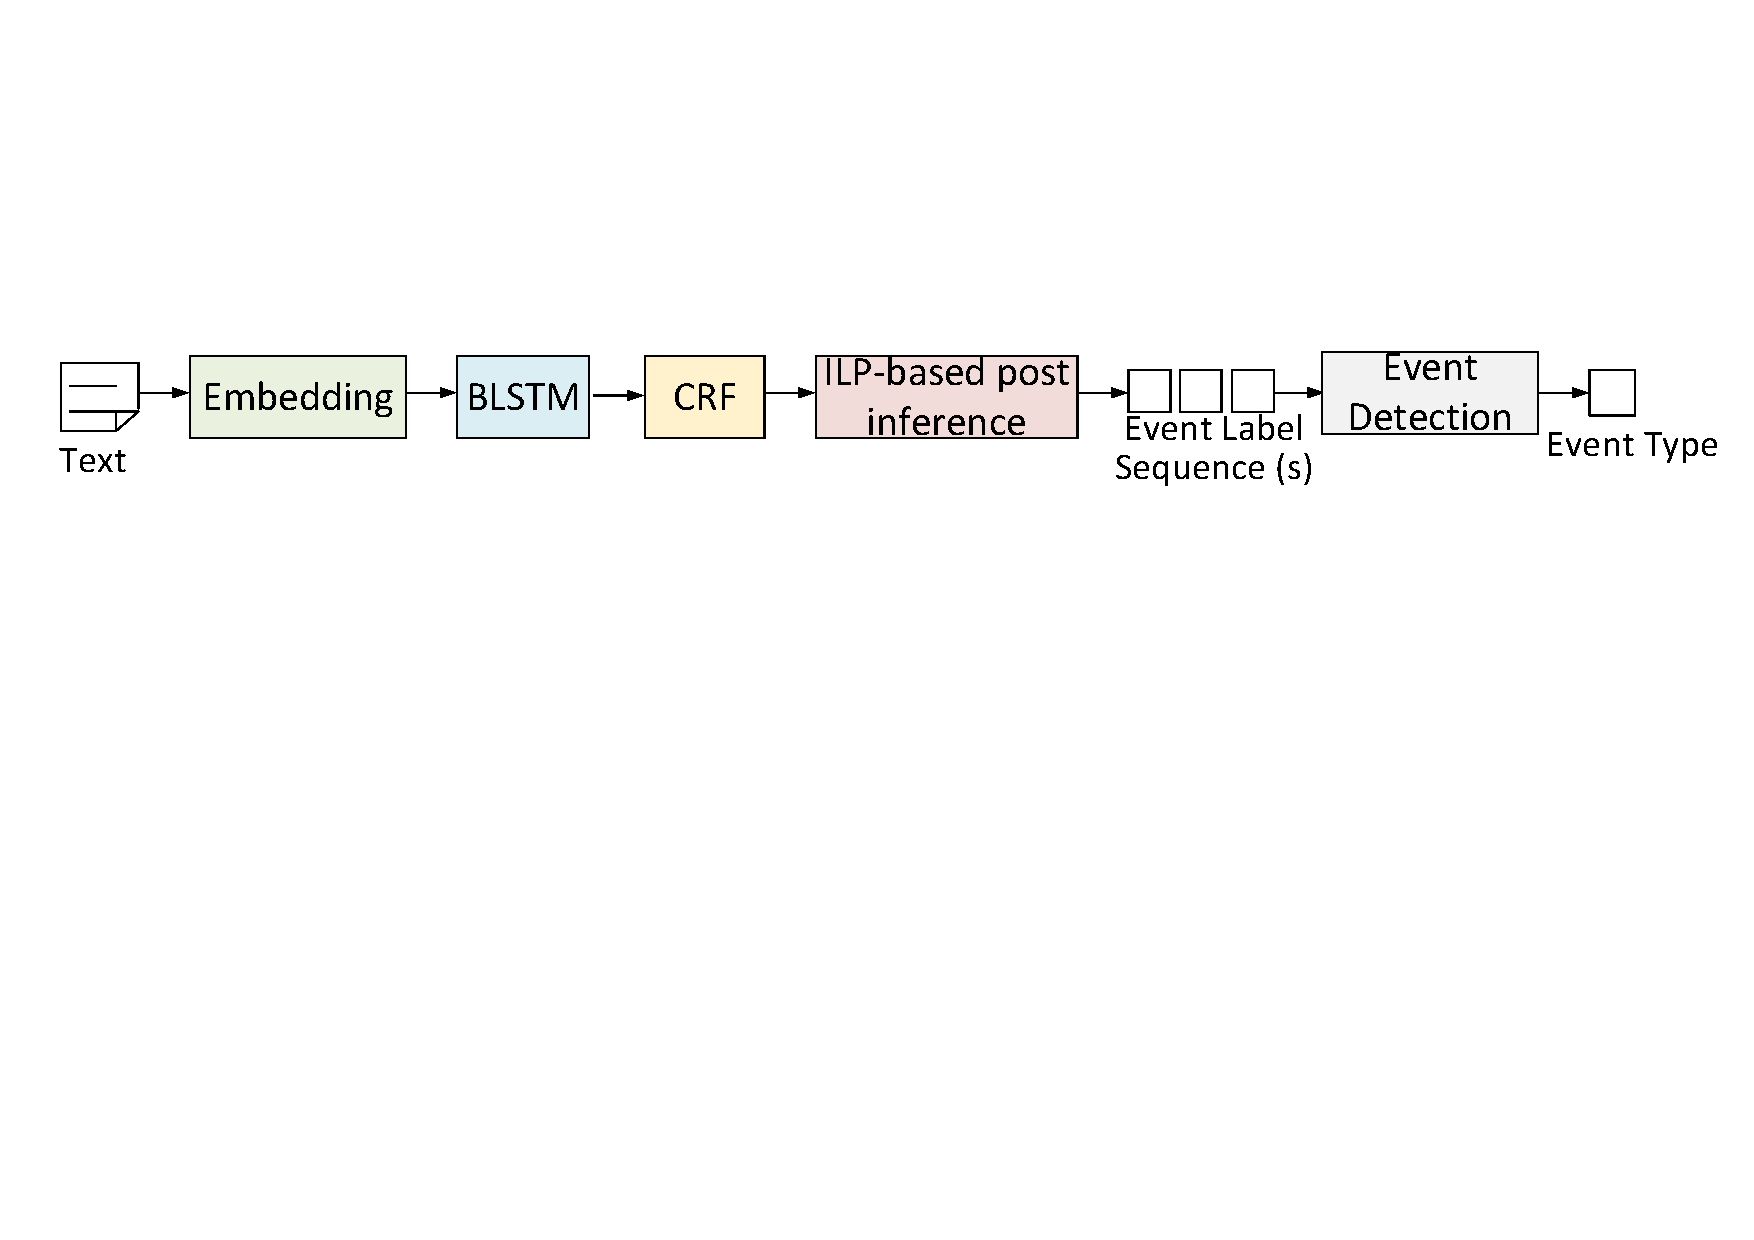
\includegraphics[width=0.5\textwidth]{figs/model.pdf}
  \vspace{-2mm}
  \caption{Our 2-stage event extraction pipeline.}\label{fig:model}
  \vspace{-2mm}
\end{figure}




\subsection{Stage 1: Key Argument and Event Detection \label{evede}}
The model used in stage 1 consists of a Bidirectional Long Short-Term Memory (BLSTM) network with a conditional random field \cite{lafferty2001conditional}  (CRF) layer
and an Integer Linear Programming (ILP) based post inference. The BLSTM-CRF layer finds the optimal labeling sequence which will then be
post-processed by an ILP solver. Using the labeling sequence, an event detector then checks if the sentence mentions a specific event.

\paragraph{BLSTM}
%The LSTM network~\cite{hochreiter1997long} is a natural fit for sequence labeling.
%, which maintains a memory based
%on historical contextual information. Formally, given a sentence $\bm{w} = \{w_1, w_2, \dots, w_n\}$ of length $n$, we use $\textbf{x}_t$
%to represent feature vector, e.g., word embeddings, corresponding to the $t$-th word $w_t$.
At each time $t$, a forward LSTM layer takes $\textbf{x}_t$ as input and computes the output vector $\overrightarrow{\textbf{h}}_t$ of the
past context, while a backward LSTM layer reads the same sentence in reverse and outputs $\overleftarrow{\textbf{h}}_t$ given the future
context. We concatenate these two vectors to form the output vector of a BLSTM, which is fed into a softmax layer to estimate a probability
distribution over all possible labels.

\paragraph{CRF}
%A straightforward way to find the label sequence for a given sentence is to
Choosing the best label for each word individually according to
the BLSTM
%with maximum probability by LSTM as the prediction for each word.
%However, this greedy strategy
ignores the dependencies between labels, thus cannot guarantee the best sequence.  %this independent labeling strategy
%is limited especially when there are strong dependencies and constraints between labels.
%To model the correlations between labels,
Therefore, we introduce a CRF layer over the BLSTM output.
% which is shown to be effective in various sequence labeling tasks~\cite{collobert2011natural,huang2015bidirectional}. %, such as POS tagging and NER .

We consider $\textbf{P}$ to be a matrix of confidence scores output by BLSTM, and the element $\textbf{P}_{i,j}$ of the matrix denotes the probability of the label $j$ for the $i$-th word in a sentence. The CRF layer takes a transition matrix $\textbf{A}$ as parameter, where $\textbf{A}_{i,j}$ represents the score of a transition from label $i$ to label $j$. The score of a sentence $\bm{w}$ along with a path of labels $\bm{y} = \{y_1, y_2, \ldots, y_n\}$ is measured by the sum of BLSTM outputs and transition scores:
\begin{equation}
	score(\bm{w}, \bm{y}) = \sum\limits_{i=0}^n\textbf{P}_{i, y_i} + \sum\limits_{i=1}^n\textbf{A}_{y_i, y_{i+1}},
\end{equation}
During test, given a sentence $\bm{w}$, we adopt the Viterbi algorithm~\cite{rabiner1989tutorial} to find the optimal label sequence with the maximum score among all possible label sequences.

\paragraph{ILP-based Post Inference}
The output sequences of BLSTM-CRF do not necessarily satisfy the structural constraints of event extraction.
%For instance, regardless of
%how many key arguments are correctly identified by BLSTM-CRF, if there is one key argument missing, this detection should be considered as failed.
%
We thus propose to apply ILP to further globally optimize the BLSTM-CRF output  to produce the best label sequence. Formally, let
$\mathcal{L}$ be the set of possible argument labels. For each word $w_i$ in the sentence $\bm{w}$ and a pair of labels $ \langle l, l'
\rangle \in \mathcal{L} \times \mathcal{L}$, we create a binary variable ${v_{i,l,l'} \in \{0, 1\}}$, denoting whether or not the $i$-th
word $w_i$ is tagged as label $l$ and its following word $w_{i+1}$ is tagged as label $l'$ at the same time. The objective of ILP is to
maximize the overall score of the variables as:
\begin{displaymath}
	\sum\nolimits_{i, l, l'}v_{i,l,l'} * (\textbf{P}_{i,l}+\textbf{A}_{l,l'}) .
\end{displaymath}
where we consider the following four constraints:

\textbf{C1}: Each word should be and only be annotated with one label, i.e.:
\begin{equation}
	\sum\nolimits_{l,l'}v_{i,l,l'}=1
\end{equation}

\textbf{C2}: If the value of $v_{i,l,l'}$ is $1$, then there has to be a label $l^*$ that will make $v_{i+1,l',l^*}$ equal to $1$, i.e.:
\begin{equation}
	v_{i,l,l'} = \sum\nolimits_{l^*}v_{i+1,l',l^*}
\end{equation}

\textbf{C3}: If the current label is \texttt{I-arg}, then its previous label must be \texttt{B-arg} or \texttt{I-arg}, i.e.:
\begin{equation}
	v_{i,\texttt{I-arg},l'} = v_{i-1,\texttt{B-arg},\texttt{I-arg}} + v_{i-1, \texttt{I-arg}, \texttt{I-arg}}
\end{equation}

\textbf{C4}: For a specific event type, all its key arguments should co-occur in the sentence, or none of them appears in the resulting sequence. For any pair of key arguments $arg_1$ and $arg_2$ with respect to the same event type, the variables related to them are subject to:
\begin{equation}
	\sum\nolimits_{i,l'}{v_{i,\texttt{B-arg}_1,l'}} \leq n * \sum\nolimits_{j,l^*}{v_{j,\texttt{B-arg}_2,l^*}}
\end{equation}
where $n$ is the length of the sentence.

\paragraph{Event Detection}
This step simply %maps the input sentence to a specific event type, checking
if the input sentence contains all the key arguments of a specific event type by
examining the labeling sequence. % produced by the ILP post-inference layer.


\paragraph{Multi-typed Events}
There are scenarios where one sentence expresses multiple events which share some key arguments,
% one event is associated with multiple types,
but most current event extractors only map a sentence to one event.
For example, in S5, \emph{Obama} is the \texttt{office\_holder} of a \texttt{government\_position\_held} event and \texttt{nominee} of an \texttt{award\_nomination} event.
\begin{quote}
	\textbf{S5}: \underline{\emph{Obama}} was  inaugurated as \underline{\emph{president}} on \underline{\emph{January}}, \underline{\emph{2009}}, and was named the  \underline{\emph{ Nobel  Peace  Prize}}  laureate nine months later.
\end{quote}
One of the advantages of our approach is that it can be easily extended to support multi-typed events.
To do so, we allow our ILP solver to output multiple optimal sequences. Specifically, after our model outputs the best sequence $\bm{s}^t$
at time $t$, we remove the previously best solutions
 $\{\bm{s}^1, \ldots, \bm{s}^{t}\}$ from the solution space, and re-run our solver to obtain the next optimal sequences $\bm{s}^{t+1}$.
We repeat the optimization procedure until the difference between the scores of $\bm{s}^1$ and $\bm{s}^T$ is greater
than a threshold $\lambda$, and consider all solutions $\{\bm{s}^1, \bm{s}^2, \ldots, \bm{s}^{T-1}\}$ as the optimal label sequences.
We use Gurobi~\cite{gurobi} as our ILP solver and set $\lambda=0.5 \times n$, which averagely produce~1.07 optimal sequences for each sentence.

\subsection{Stage 2: Non-key Argument Detection}
After event detection, a sentence will be classified into one or more event types, and labeled with the corresponding key arguments.
%The next step is argument detection, which
%Next, we will identify the remaining non-key arguments in the sentence.
%
We next adopt the same BLSTM-CRF architecture %(that is used for event detection)
to detect the remaining non-key arguments, where we encode the key-argument label (from the first stage) %(output of event detection)
of each word into a key-argument feature vector through a look-up table, and concatenate it with the original word
embedding as the input to a new BLSTM-CRF. Note that we do not need post inference here, because there is no structural constraints between non-key arguments.
% \FIXME{because...}.
